\chapter*{‌پیوست}
\markboth{پیوست}{}

% براي شماره‌گذاري روابط، جداول و اشكال موجود در پيوست‌ از ساختار متفاوتي نسبت به متن اصلي استفاده مي‌شود كه در زير به‌عنوان نمونه نمايش داده شده‌است. 

\section*{کد‌ها و پیوست‌ها}
تمامی‌ کد‌ها و پیوست‌های پروژه نظیر ساختار پایگاه‌داده، نیازمندی‌های اجرا و فایل‌های قابل اجرا در مخزن زیر در دسترس است.
\begin{latin}
	\href{https://github.com/smf8/30bird}{\lr{https://github.com/smf8/30bird}}
\end{latin}

\section*{نمودار‌های رابطه-موجودیت}

\begin{figure}
	\centering
	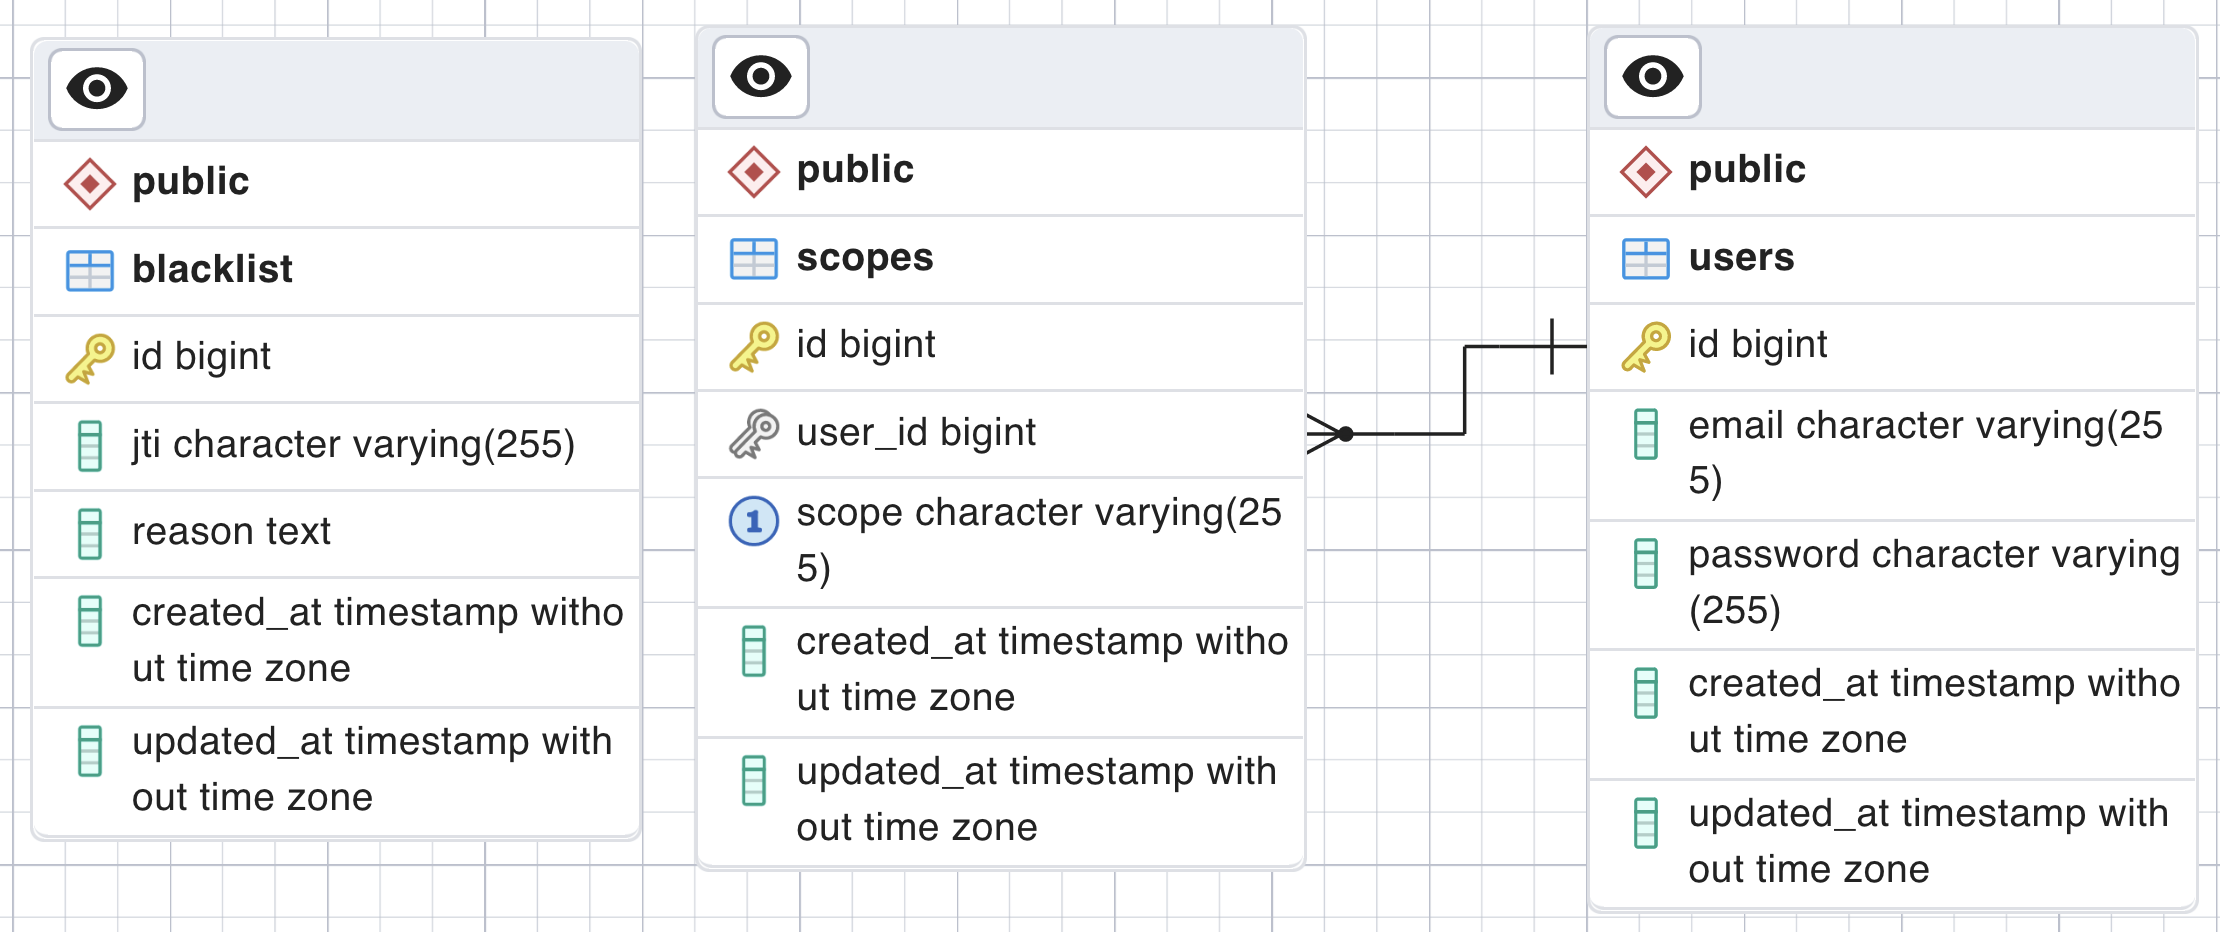
\includegraphics[width=0.9\linewidth]{figures/erd-ghofl}
	\caption{ساختار موجودیت‌ها و رابطه‌ها در پایگاه داده قفل}
	\label{fig:erd-ghofl}
\end{figure}

\begin{figure}
	\centering
	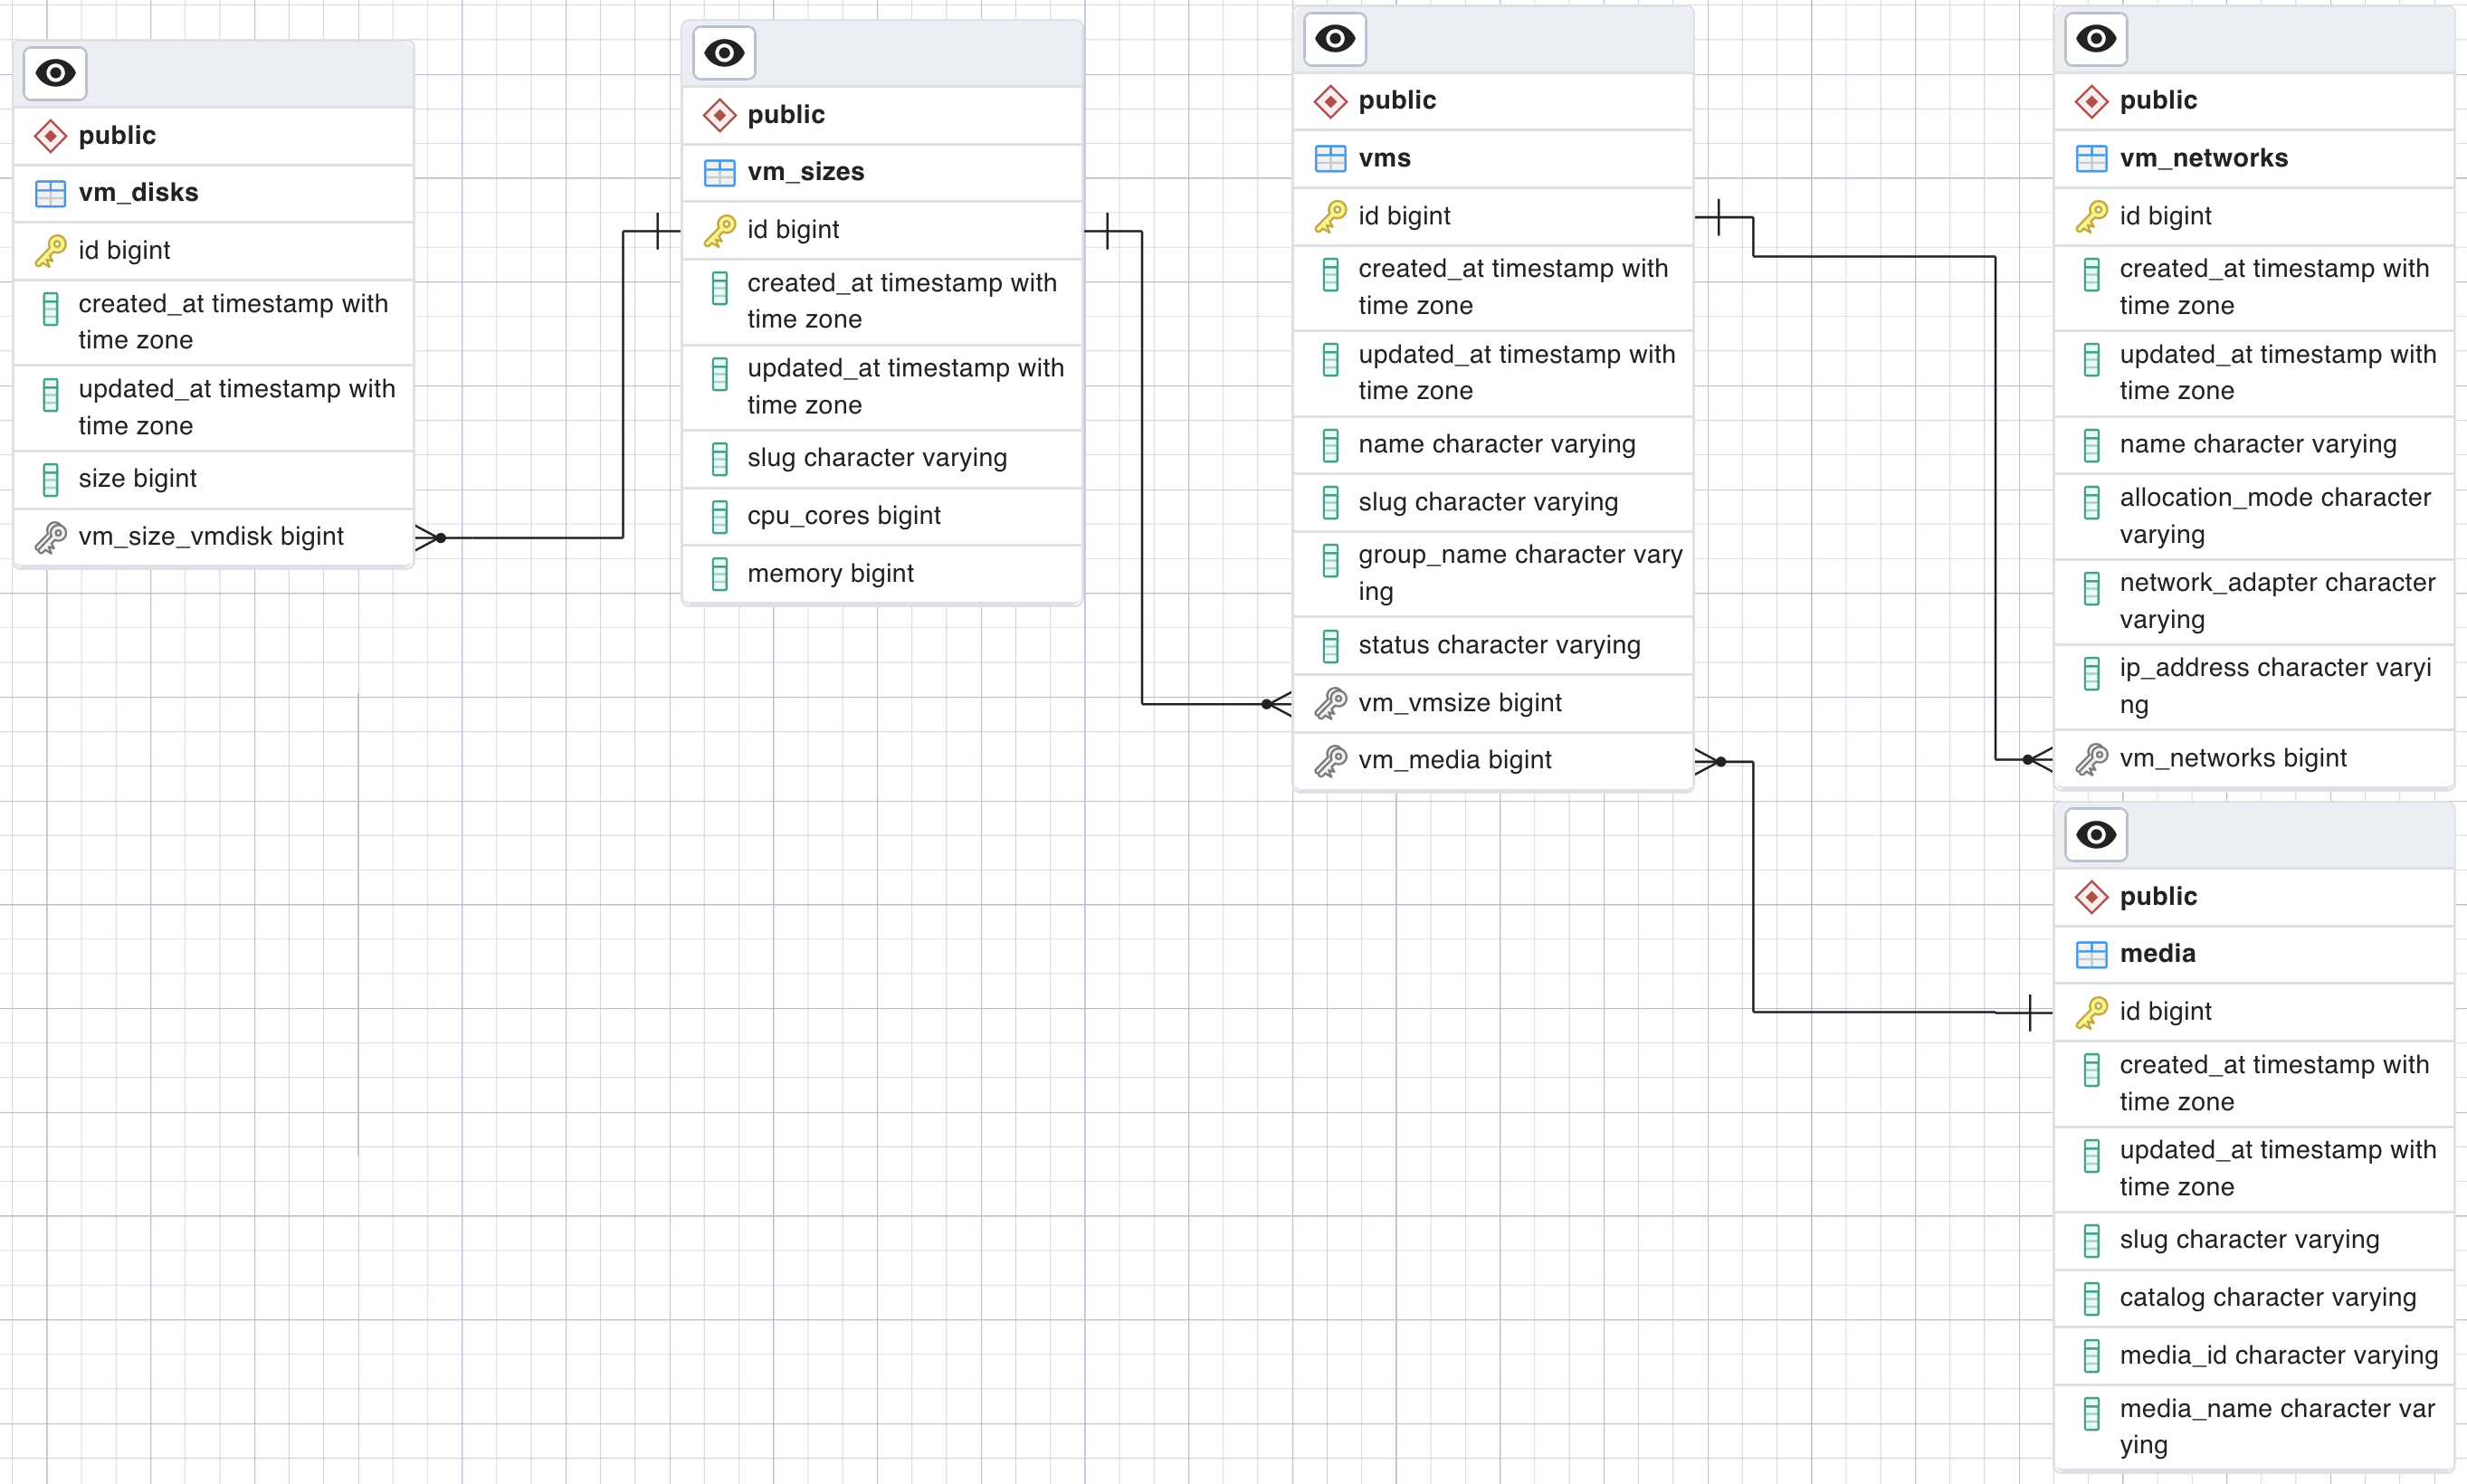
\includegraphics[width=1\linewidth]{figures/erd-baaje}
	\caption{ساختار موجودیت‌ها و رابطه‌ها در پایگاه داده باجه}
	\label{fig:erd-baaje}
\end{figure}

\begin{figure}
	\centering
	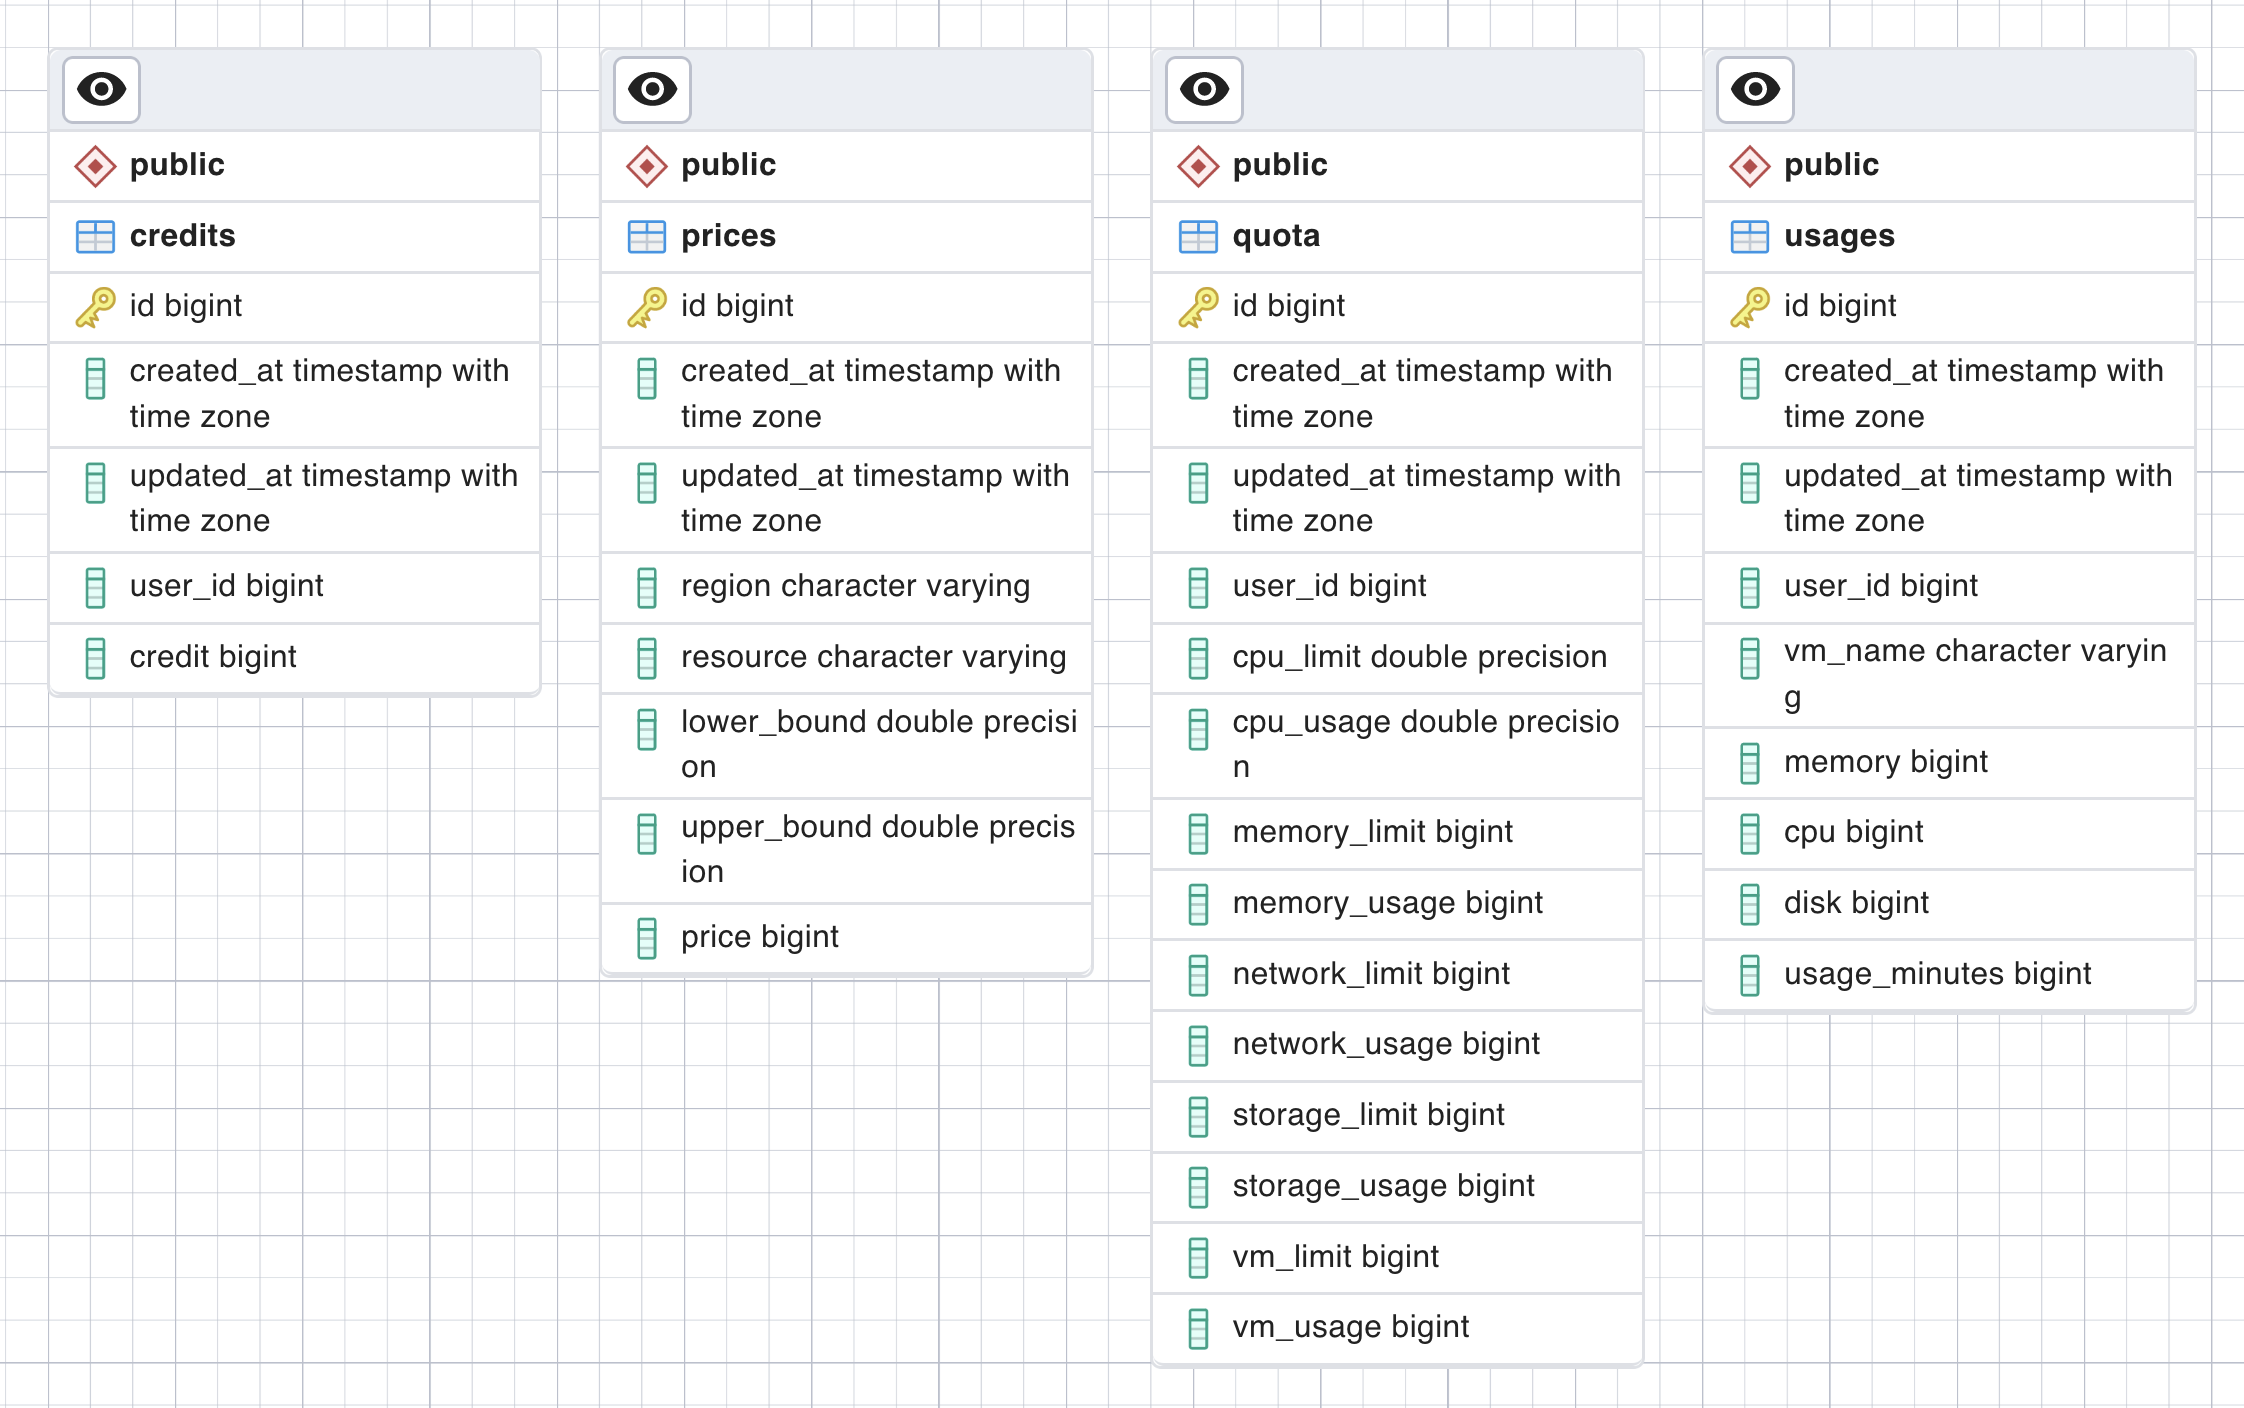
\includegraphics[width=\linewidth]{figures/erd-nazem}
	\caption{ساختار موجودیت‌ها در پایگاه داده ناظم}
	\label{fig:erd-nazem}
\end{figure}

\section*{نمودار‌های توالی}

نمونه‌ای از عملیات‌های توالی\LTRfootnote{Sequence Diagram} در زیر قرار داده شده‌است.

\begin{figure}
	\centering
	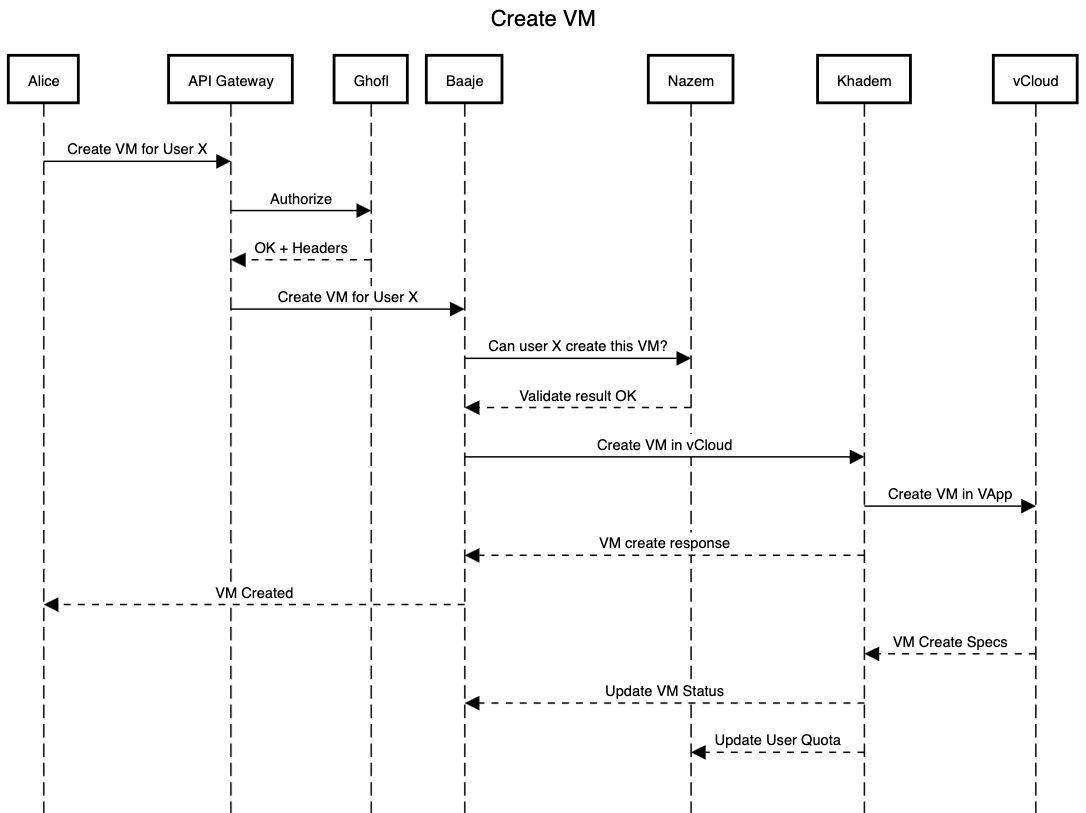
\includegraphics[width=1\linewidth]{figures/create-vm-sequence}
	\caption{نمودار توالی ایجاد یک ماشین مجازی}
	\label{fig:create-vm-sequence}
\end{figure}
\begin{figure}
	\centering
	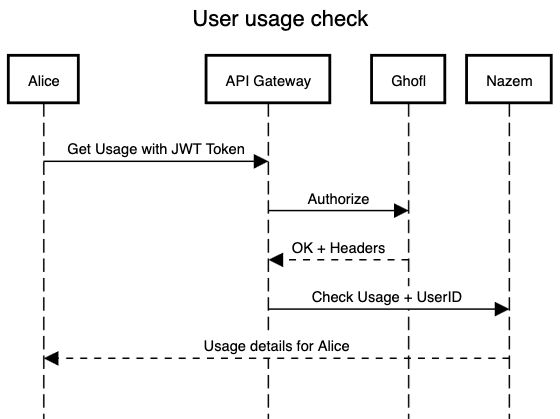
\includegraphics[width=1\linewidth]{figures/user-usage-sequence}
	\caption{نمودار توالی دریافت جزئیات مصرف منابع کاربر}
	\label{fig:user-usage-sequence}
\end{figure}

